%%%%%%%%%%%%%%%%%%%%%%%%%%%%%%%%%%%%%%%%%%%%%%%%%%%%%%%%%%%%%%%%%%%%%%%%%%%%%%
%                  Latex Vorlage f\"{u}r Abschlu{\ss}arbeiten                        %
%%%%%%%%%%%%%%%%%%%%%%%%%%%%%%%%%%%%%%%%%%%%%%%%%%%%%%%%%%%%%%%%%%%%%%%%%%%%%%
\documentclass[12pt,a4paper,DIV13,pdftex,BCOR10mm,fleqn,liststotoc,bibtotoc,cleardoubleempty]{scrbook}
%,footexclude,headexclude standard,chapterprefix,dvips
\usepackage{times}            %Font
\usepackage[latin1]{inputenc} %erkennt \"{a},\"{o},\"{u}
\usepackage{german,amsfonts}  %erkennt \3 als {\ss}
\usepackage[T1]{fontenc}      %z.B. f\"{u}r (besseres) automatisches Trennen nach Umlauten
% \usepackage{latexsym}         %sonstige Symbole (\partial)
\usepackage{graphicx}         %[draft]
%\usepackage[a4,center]{crop}  % cam,frame, habe D:\texmf\dvips\config\config.ps angepa{\ss}t!!!
%\usepackage{pstricks,pst-node,pst-tree,pst-plot}  %um B\"{a}ume zu zeichnen
\usepackage{booktabs}         %f\"{u}r sch\"{o}nere Tabellen
\usepackage{textcomp}         %f\"{u}r \textperthousand = promille
\usepackage{placeins}         %verhindert Gleiten von Abbildungen (bis \FloatBarrier)
\usepackage{amsmath} %F\"{u}r Formeln
\usepackage[breaklinks,pdfborder={0 0 0}]{hyperref} %f\"{u}r Links im PDF
\usepackage{xcolor,soul} %F\"{u}r Matlab/Octave
\usepackage{url} %f\"{u}r Hyperlinks im Literaturverzeichnis,alternativ  "hyperref" und "breakurl" [hyphens]
\usepackage{listings}         %fuer C-Programme
\usepackage{scrlayer-scrpage}%[automark] f\"{u}r Kopfzeilen
% \setheadsepline{0.4pt} %
\pagestyle{scrheadings} %Linie in Kopfzeilen
\addtolength{\topmargin}{5mm} %gesamten Text auf der Seite nach unten schieben
%\usepackage{setspace} Zeilenabstand \"{a}ndern. H\"{a}nde weg! Vergr\"{o}{\ss}ert auch den Abstand von Bildunterschriften...
%\onehalfspacing

\lstset{language=C,
basicstyle=\ttfamily\footnotesize,
keywordstyle=\color{blue},
commentstyle=\color{green},
stringstyle=\color{red},
numbers=left,
stepnumber=1,
numbersep=5pt,
%numberstyle=\tiny,
breaklines=true,
breakautoindent=true,
postbreak=\space,
tabsize=2,
showspaces=false,
showstringspaces=false,
extendedchars=true,
backgroundcolor=\color{black!10},
captionpos=b }

%%%%%%%%%%%%%%%%%%%%%%%%%%%%%%%%%%%%%%%%%%%%%%%%%%%%%%%%%%%%%%%%%%%%%%%%%%%%%%
%%%%%%%%%%%%%%%%%%%%%%%%%%%%%%%%%%%%%%%%%%%%%%%%%%%%%%%%%%%%%%%%%%%%%%%%%%%%%%
\begin{document}
%%%%%%%%%%%%%%%%%%%%%%%%%%%%%%%%%%%%%%%%%%%%%%%%%%%%%%%%%%%%%%%%%%%%%%%%%%%%%%
%%%%%%%%%%%%%%%%%%%%%%%%%%%%%%%%%%%%%%%%%%%%%%%%%%%%%%%%%%%%%%%%%%%%%%%%%%%%%%
\frontmatter
%von http://studiy.tu-cottbus.de/projektwiki/wissen:latex:diplomarbeit
\titlehead{%  {\centering Seitenkopf}
  {Hochschule f\"{u}r angewandte Wissenschaften\\
   Fachhochschule W\"{u}rzburg-Schweinfurt\\
   Fakult\"{a}t Informatik und Wirtschaftsinformatik}}
\subject{Projektarbeit}
\title{Naolympics\\[10mm]}
\subtitle{\normalsize{vorgelegt an der Hochschule f\"{u}r angewandte Wissenschaften Fachhochschule W\"{u}rzburg-Schweinfurt in der Fakult\"{a}t Informatik und Wirtschaftsinformatik zum Abschluss eines Studiums im Studiengang Informatik}}
\author{Nils G\"obel\\Johannes Gehring\\Luca Klingert\\Michael Schmitt}
\date{\normalsize{Eingereicht am: Datum}}
\publishers{
  \normalsize{Erstpr\"{u}fer: Prof. Dr. Arndt Balzer} \\
  \normalsize{Zweitpr\"{u}fer: Prof. Dr. Daniel Kulesz}\\
}

%\uppertitleback{ }
%\lowertitleback{ }

\maketitle

\thispagestyle{empty}
\section*{Selbstst\"{a}ndigkeitserkl\"{a}rung}
Hiermit versichere ich, dass ich die vorgelegte Bachelorarbeit/Masterarbeit selbstst\"{a}ndig verfasst und noch nicht anderweitig zu Pr\"{u}fungszwecken vorgelegt habe. Alle benutzten Quellen und Hilfsmittel sind angegeben, w\"{o}rtliche und sinngem\"{a}{\ss}e Zitate wurden als solche gekennzeichnet.\\[15mm]
%% Abstand und Linie
\vspace{20mm}
\hrule
\vspace{5mm}
W\"urzburg, den \date{Datum}

\cleardoublepage     % min. eine Freiseite

\thispagestyle{empty}
\section*{Kurzfassung}
In dieser Arbeit geht es um ...

\vspace{5cm}
\section*{Abstract}
This thesis is about ....

\nonfrenchspacing
\renewcommand{\figurename}{Abb.}
\renewcommand{\tablename}{Tab.}

%\setcounter{page}{7}%  {tocdepth}{1} =section
%\lstset{language=C, basicstyle=\ttfamily\small, commentstyle=\itshape}
%\automark[chapter]{chapter} ???

\tableofcontents %
\listoffigures %
\listoftables
%%%%%%%%%%%%%%%%%%%%%%%%%%%%%%%%%%%%%%%%%%%%%%%%%%%%%%%%%%%%%%%%%%%%%%%%%%%%%%
%%%%%%%%%%%%%%%%%%%%%%%%%%%%%%%%%%%%%%%%%%%%%%%%%%%%%%%%%%%%%%%%%%%%%%%%%%%%%%
%%%%%%%%%%%%%%%%%%%%%%%%%%%%%%%%%%%%%%%%%%%%%%%%%%%%%%%%%%%%%%%%%%%%%%%%%%%%%%
%%%%%%%%%%%%%%%%%%%%%%%%%%%%%%%%%%%%%%%%%%%%%%%%%%%%%%%%%%%%%%%%%%%%%%%%%%%%%%
\mainmatter
%\include{kap1.tex}
\chapter{Einleitung}
\section{Theoretische Grundlagen}
Wichtiger Teil des Spiel- bzw. Programmablaufs ist die Erkennung des gespielten Spiels und im Anschluss die kontinuierliche Auswertung
des Spielstands. Dies soll in diesem Projekt rein \"uber die Stirnkamera der Roboter sowie \textit{Computer Vision (CV)} Algorithmen erfolgen.
Eine andere M\"oglichkeit w\"are, die Roboter untereinander über das Netzwerk, bspw. HTTP, über getätigte Spielzüge und damit den Spielstand
kommunizieren zu lassen. Problem hierbei ist einerseits, dass man hier ggf. nicht komplett auf \textit{CV} verzichten kann, um z.B. das Spiel
zu Beginn zu erkennen, andererseits, dass bei \textit{Mensch vs. NAO} logischerweise eine andere andere Form der Kommunikation gewählt werden
müsste, etwa über die \textit{TextToSpeech} -Funktion des \textit{NAO}. Eine zweite Möglichkeit, dieses Problem zu lösen, wäre, wenn die Spiele-
App die Kommunikation mit den Robotern übernimmt, oder der menschliche Spieler seinen Zug zusätzlich über einen zweiten Computer einträgt und so
mitteilt. Dies würde jedoch gleichzeitig den Gedanken verletzen, dass die Roboter völlig selbstständig spielt und handelt, wozu eben nicht nur die
Bedienung des Touchscreens gehören, sondern auch Dinge wie die Spielstanderkennung und -auswertung. Anders könnte man all diese Aufgaben an ein anderes
Gerät \dq outsourcen\dq und dem \textit{NAO} nur mitteilen, wie er sich zu bewegen hat, was einer Marionette gleicht. Daher die Entscheidung,
die Erkennung über \textit{CV} Algorithmen zu realisieren. Hierfür wurden weitestgehend Standardverfahren der \textit{Computer Vision} verwendet, welche
nachfolgend theoretisch erörtert werden. Für die Implementierung wurde die Open Source Bibliothek OpenCV verwendet\cite{opencv_library}.

\subsection{Bildverarbeitung}
Unter realen Bedingungen, wie etwa inkonsistenter Beleuchtung, treten einige Probleme auf, welche die Weiterverarbeitung von Bildern deutlich erschweren 
können. Bei schlechten Lichtbedingungen beispielsweise neigen Aufnahmen zu viel Rauschen (eng. \textit{Noise}) im Bild, also Pixeln mit fehlerhaften Bildwerten\cite{CAVE_0394}.
Ein anderes Problem, was aber im Kontext dieses Projektes keine nennenswerte Rolle spielt, ist sog. \textit{Bewegungsunschärfe}, bei der sich das Objekt während 
der Aufnahme bewegt und so unscharf und \dq verschmiert\dq auf dem Bild erscheint\cite[S.\. 43]{Klette14}. Bei Bildschirmaufnahmen und computergrafisch gerenderten Szenen treten solche
Effekte logischerweise weniger bis gar nicht auf. Ziel ist es also, ein Bild so zu verarbeiten, dass in nachfolgenden Anwendungen, wie etwa Objekterkennung
diese negativen Effekte möglichst wenig ins Gewicht fallen. Gängige Vorgehensweise ist hierbei die Kombination von Weichzeichnen (eng. \textit{smoothing}) und
ein Kantenerkennungsalgorithmus. Wir erhalten daraus ein verarbeitetes Bild $J$.

%//TODO: auch was über Deep Learning/Machine Learning als Erkennung reinschreiben 

\subsubsection*{Weichzeichnen}
Weichzeichnen (engl. \textit{smoothing}) zielt darauf ab, \dq Ausreißer\dq, also Rauschen im Bild $I$ zu reduzieren\cite{Klette14}. Hierfür wird allermeistens eine lokale Operation in einem
$(2k+1) \times (2k+1), \; k \in \mathbb{N} $ großen Fenster $W$ durchgeführt, wobei jeder Pixel des Bildes besucht und als Referenzpixel im Zentrum des Fensters
sitzend betrachtet wird. Innerhalb dieses Fensters wird dann eine lokale Operation durchgeführt, und ein neuer Pixelwert $J(p)$ für das Referenzpixel berechnet wird, 
wobei nur die Pixel innerhalb des Fensters einbezogen werden. Die Operation kann entweder \textit{linear} oder \textit{nicht-linear} erfolgen. 
Bei einer \textit{nicht-linearen lokalen Operation} wird ein Algorithmus auf die Pixel angewendet, welcher keiner Faltung entspricht, beispielsweise eine Maximum-Operation\cite[S.\. 46]{Klette14}.
\begin{align}
    J(p) = \max\{I(x+i, y+j): -k \le i \le k \wedge -k \le j \le k\}
\end{align}

Eine \textit{lineare lokale Operation} lässt sich durch eine diskrete Faltung des \textit{gleitenden Fensters} $W$ (auch Kernel oder Maske genannt) mit $I$ beschreiben. Für den Pixel $p = (x,y)$ lautet die Formel
wie folgt: 
\begin{align}
    J(p) = W_p \ast I(p) = \frac{1}{S} \sum_{i=-k}^{i=k}\sum_{j=-k}^{j=k} w_{i,j} \cdot I(x+i, y+j)
\end{align}
Mit Gewichten $w_{i,j} \in W$ und Skalierungsfaktor $S$ (i.d.R. $\sum w_{i,j}$)\cite[S.\. 47]{Klette14}.

Beliebte Kernel für das Weichzeichen sind der Mittelwert-Filter, auch Box-Filter genannt, sowie der Gaussfilter. Ersterer berechnet innerhalb von $W$ den Mittelwert und somit auf das ganze Bild gesehen
den gleitenden Mittelwert. Der Gaussfilter approximiert eine zweidimensionale Gaussfunktion, üblicherweise mit $\mu_x = 0, \mu_y = 0$, sodass der Peak der Funktion im Zentrum des Fensters liegt\cite[S.\. 57f.]{Klette14}.

\begin{align}
    \begin{bmatrix}
        1 & 1 & 1 \\
        1 & 1 & 1 \\
        1 & 1 & 1
    \end{bmatrix} 
    \frac{}{9}
    & \qquad \qquad \qquad
    \begin{bmatrix}
        1 & 4 & 7 & 4 & 1 \\
        4 & 16 & 26 & 16 & 4\\
        7 & 26 & 41 & 27 & 7\\
        4 & 16 & 26 & 16 & 4\\
        1 & 4 & 7 & 4 & 1 
    \end{bmatrix} 
    \frac{}{273}\\
    \text{Box-Filter}(k = 1) & \qquad \qquad \qquad \text{Gaussfilter}(k = 2, \sigma = 1)\notag
\end{align}
\begin{figure}[htbp]
    \centering
    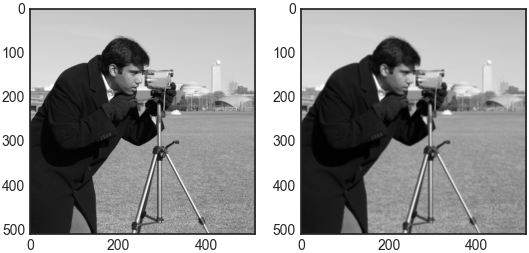
\includegraphics[width=15cm]{bilder/gaussian_k3_s1.png}
 %[width=60mm], [height=60mm], [scale=0.75], [angle=45,width=52mm], ....
    \caption[Beispiel Weichzeichnen]{Links: Unbarbeitetes Bild, Rechts: Weichgezeichnetes Bild (Gaussfilter, $k = 2, \sigma = 1$)}
    \label{fig:smoothing}
    \end{figure}

\subsubsection*{Kantenerkennung}
Eine Kante in einem Bild wird im sog. \textit{Stufenkantenmodell} als rapider Intensitätsunterschied innerhalb eines kleinen räumlichen Bereichs definiert. Hierbei muss man jedoch beachten,
dass das gleiche auch für Rauschen gilt. Kanten bzw. Kantenbilder (engl. \textit{edge maps}) können den Inhalt eines Bildes einfangen und simplifizieren, indem nur die Konturen der Objekte
behalten werden und \" nicht-Kanten \" verworfen werden. So lassen sich auch Umwelteinflüsse wie wechselnde Beleuchtung reduzieren bis eliminieren\cite[S.\. 10f.]{Klette14} 
Viele Kantenerkennungsalgorithmen basieren auf dem Stufenkantenmodell (\textit{Sobel, Canny, Laplace, Meer-Georgescu}), um nur die Bildbereiche zu erfassen, welche eine solche Stufenkante repräsentieren,
und nutzen hierfür den approximierten Gradienten des Pixels $p = (x,y)$. Der Gradient

\begin{align}
    \nabla I = \mathbf{grad}\, I = \left[ \frac{\partial I}{\partial x}, \frac{\partial I}{\partial y} \right]^T \approx \left[ I_x, I_y \right]
\end{align}

welcher die approximierten ersten Ableitungen nach $x$ und $y$, $I_x \approx \frac{\partial I}{\partial x}, I_y \approx \frac{\partial I}{\partial y}$ enthält.
Diese lassen sich mit verschiedenen Kerneln ermitteln, beispielsweise dem Sobel-Operator:

\begin{align}
    & \qquad \begin{bmatrix}
        -1 & 0 & 1 \\
         -2 & 0 & 2 \\
        -1 & 0 & 1
    \end{bmatrix} && \qquad
    \begin{bmatrix}
        -1 & -2 & -1 \\
         0 & 0 & 0 \\
        1 & 2 & 1
    \end{bmatrix}\\
    & \text{Sobel-Op. }x\text{-Richtung}(k=1) && \text{Sobel-Op. }y\text{-Richtung}(k=1)\notag
\end{align}

Wichtige Parameter für Kantenerkennung mit Gradienten sind die Länge bzw. der Betrag des Gradienten $g(p)$ sowie dessen Richtung $\Theta(p)$:

\begin{align}
    g(p)& = \| \mathbf{grad}\, I(p) \|_2 = \sqrt{I_x^2 + I_y^2}\\
    \Theta(p)& = \mathrm{atan2}(I_y, I_x)
\end{align}

Ein weiteres Modell für die Definition einer Kante, hier nicht näher besprochen, in einem Bild ist das \textit{Phasenkongruenzmodell}, beispielsweise im \textit{Kovesi}-Algorithmus\cite[S.\.79ff.]{Klette14}.
\\
\\
\textbf{Canny-Algorithmus} Der Canny-Algorithmus verbindet die bereits vorgestellten Bildverarbeitungskonzepte zu einem robusten Kantenerkennungsalgorithmus, wobei er ein binäres Kantenbild erzeugt. 
Hierfür nutzt der Algorithmus den Gaussfilter, den Gradienten, eine sog. \textit{non-maxima suppression} und einen Hysterese-basierten \textit{edge-following} Ansatz.
\newpage
\begin{algorithm}[htbp]
% \vspace{-7cm}
    \LinesNumbered
    \SetAlgoLined
    \caption{Canny-Algorithmus nach \cite[S.\. 64]{Klette14}}\label{alg:one}
    \KwData{Image $I$, Lower Threshold $T_{low}$, Upper Threshold $T_{high}$, $\sigma > 0$}
    \KwResult{edge map $J$}
    Smooth $I$ with Gaussian filter $G_\sigma$;\\
    Calculate approx. gradient $\mathbf{grad} I(p)$ as well as $\Theta(p)$ and $g(p)$;\\
    Round $\Theta(p)$ to multiples of $\frac{\pi}{4}$;\\
    \textit{non-maxima suppression}:\\
    \For{every pixel $p$}{
        compare $g(p)$ with the two neighbors' $g(q), g(q')$ in direction $\Theta(p)$;\\
        \If{$g(p) \le g(q)$ or $g(p) \le g(q')$}{$g(p) = 0$}
    }
    \textit{edge-following}:\\
    \For{every pixel $p$ not visited}{
        \If{$g(p) \ge T_{high}$}{
        Mark $p$ as edge pixel;\\
        Visit all 8-adjacent neighbors $q$ of $p$;\\
        \If{$g(q) > T_{low}$}{
            Mark $q$ as edge pixel;\\
            $q = p$;\\
            \textbf{Go to} $15$;
        }
        }
    }
\end{algorithm}

\vspace{\baselineskip}
% \vspace{1cm}
Bei der \textit{non-maxima suppression} vergleichen wir den gerade besuchten Pixel $p = (x,y)$ mit seinen direkten Nachbarn in der gerundeten Richtung des Gradienten $\Theta(p)$. Wenn beispielsweise $\Theta(p) = \frac{\pi}{2}$, so zeigt der Gradient in die vertikale Richtung und wir vergleichen $g(p) = g(x,y)$ mit $g(x, y-1)$ und $g(x,y+1)$.\\
Beim \textit{edge-following} wenden wir einen Hysterese-Ansatz an, indem wir die \dq Pfade\dq an Pixeln verfolgen, deren direkte Nachbarn einen der beiden Schwellenwerte $T_{low}$ oder $T_{high}$ überschreiten. Man erhält durch den Canny-Algorithmus somit kein vollständig binärisiertes Bild, aber durch die \textit{non-maxima suppression} werden lediglich die relevanten Kantenpixel in $J$ erhalten\cite[S.\. 64]{Klette14}.\\

\textbf{Morphologische Operationen} \textit{OpenCV} spricht bei einer lokalen Minimum-Operation von \textit{erosion} und bei einer lokalen Maximum-Operation von \textit{dilation}. Diese können dabei helfen, Kanten in Kantenbildern zu verbreitern oder zu schmälern und somit die Konturen zu \dq schärfen \dq \cite{learning_opencv}.

\subsection{Hough-Transformation}
Die Hough-Transformation ist ein einfache und zuverlässige Methode, Linien und Kreise in Bildern  zu erkennen. Hierfür wird für das Bild $I$ im \textit{Bildraum} ($(x,y)$-Koordinaten) ein \textit{Parameterraum} aufgespannt. Die Art und Anzahl der Parameter wird dabei von der zu erkennenden Geometrie bestimmt:

\textbf{Linien} Linien werden durch die Formel
\begin{align}
    y = & ax+b
\end{align}
parametrisiert. Betrachtet man nun einen Punkt bzw. ein Pixel $p$ auf einer Linie, so erhält man:
\begin{align}
    y_p & = ax_p + b\\
    b & = -ax_p + y_p
\end{align}
Eine weitere Möglichkeit, Linien zu parametrisieren, welche für Bilder besser geeignet ist, da sie die das Intervall der Parameter begrenzt, ist über die sinusoidale Darstellung:
\begin{align}
    0 = & x \sin \Theta - y \cos \Theta + \rho
\end{align}
mit dem Winkel zwischen $x$-Achse und Linie $\Theta$ und dem Abstand $\rho$ zwischen Pixel $p = (x,y)$ und dem Ursprung $(0,0)$.

\begin{figure}[htbp]
    \centering
    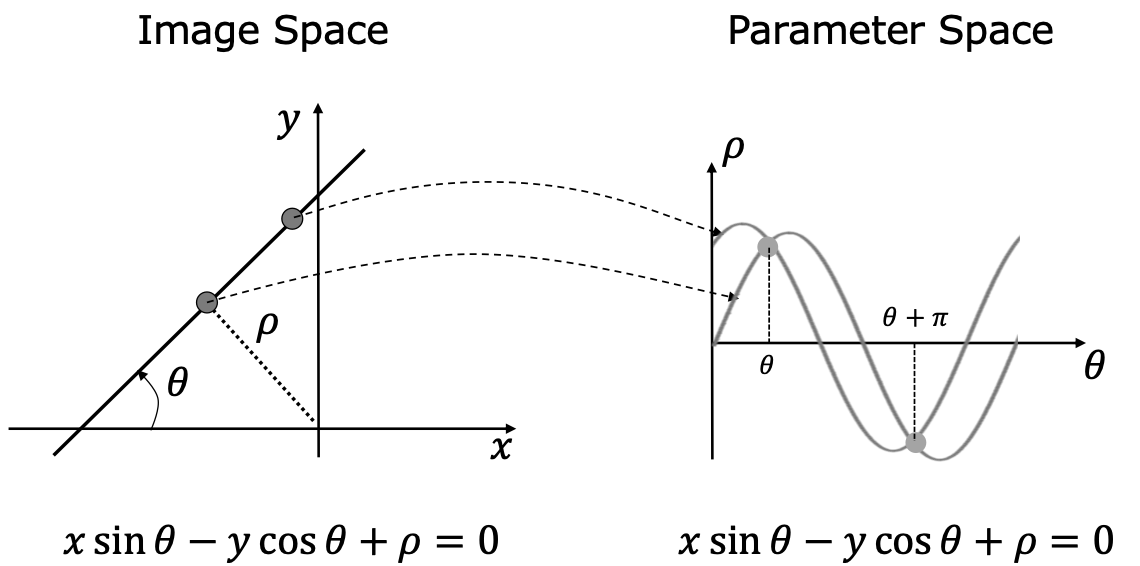
\includegraphics[width=12cm]{bilder/hough_line_space.png}
    \caption[Parameterraum Linie Sinusoid]{Linie als Parameter von Sinusoiden dargestellt \cite{nayar_boundary_detection}}
    \label{fig:hough_line_space}
\end{figure}

Es lässt sich erkennen, dass eine Linie im Parameterraum $(a,b)$ bzw. $(\Theta, \rho)$ alle Linien im Bildraum darstellt, die den Pixel $p$ schneiden\cite{nayar_boundary_detection}.\\

\textbf{Kreise} Kreise lassen sich durch die Formel
\begin{align}
    (x_p - a)^2 + (y_p - b)^2 = r^2
\end{align}
beschreiben, mit dem Mittelpunkt $(a,b)$ und Radius $r$. Somit ergibt sich bei bekanntem Radius $r$ der Parameterraum $(a, b)$ und für unbekannte Radii $(a, b, r)$.\\
\newpage
\begin{figure}[htbp]
    \centering
    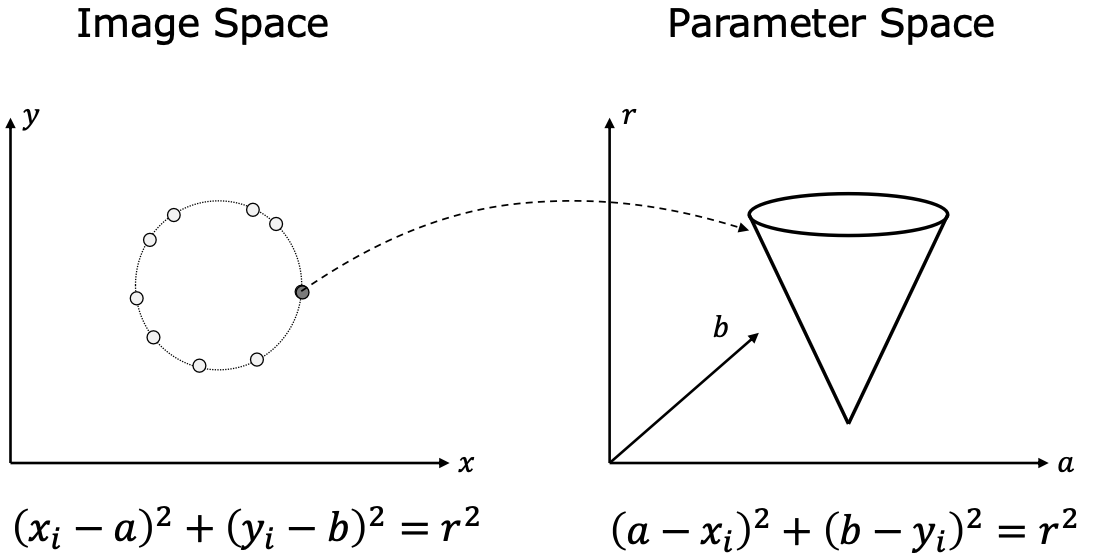
\includegraphics[width=12cm]{bilder/hough_circle_space.png}
    \caption[Parameterraum Kreise]{Kreiserkennung mit unbekanntem Radius im Parameterraum dargestellt \cite{nayar_boundary_detection}}
    \label{fig:hough_circle_space}
\end{figure}

Jeder Kreis bzw. Schicht des mit $r$ wachsenden Kegels, wie in \ref{fig:hough_circle_space} zu sehen, im Parameterraum (je nach dem ob $r$ bekannt ist) ergibt somit einen Kreis im Bildraum, welcher den Punkt $p$ schneidet\cite{nayar_boundary_detection}.\\

\textbf{Akkumulator-Array} Mit diesem Vorwissen über Kreise und Linien lässt sich nun eine Methodik aufstellen, wie man Linien und Kreise in Bildern erkennt. Punkte auf einer Geraden bzw. Kreis in einem Bild werden alle als eigene Linie bzw. Kreis im Parameterraum dargestellt. Diese werden sich in dem Punkt im Parameterraum schneiden, welcher die Linie oder den Kreis im Bildraum darstellt. Wir diskretieren nun den Parameterraum $(a,b)$ (und ggf. $r$) in geeigneter Weise und erzeugen ein zwei- bzw. dreidimensionales Array mit entsprechender Größe, Akkumulator-Array $A(a,b)$ genannt, welches den diskreten Parameterraum repräsentiert und mit Zellen mit dem Wert $0$ initialisiert wird. Jeder Punkt im Bildraum ist eine Linie/Kreis im Parameterraum und verläuft diese durch die Zelle in $A$, so wird der Wert der Zelle inkrementiert. Wenn man nun für jeden Punkt $p$ in $I$ (üblicherweise ist $p$ ein Kantenpixel in einem Kantenbild) eine Linie/Kreis in $A$ \dq einträgt \dq , so ergeben die Zellen in $A$ mit den höchsten Werten die Parameter der Linien/Kreise in $I$. Es ist üblich, einen Schwellenwert $T$ für die Entscheidung Linie oder keine Linie heranzuziehen\cite{nayar_boundary_detection} \cite[S.\. 121ff.]{Klette14}.\\


\subsection{Border Tracing}
\textit{Border Tracing} oder \textit{-- Following} beschreibt eine fundamentale Technik der Analyse von Binärbildern, bei der man miteinander verbundene, \dq 1 \dq - Komponenten ermittelt und somit topologische Eigenschaften des Bildes analysiert. Hierbei erhält man meist die Konturen von Objekten im Bild. Es ist weiterhin möglich bzw. erwünscht, auch Sub-Konturen, also Grenzen innerhalb von Grenzen zu ermitteln. Die Anwendungsbereiche liegen hier bei Bild- bzw. Objekterkennung, aber auch Kompressionsmethoden\cite{suzuki_contour}. Ein Ansatz hierfür ist das Folgen von Grenz-Pixeln in einer definierten Nachbarschaft, z.B. Vier (engl. \textit{4-adjacency}), sowie einer Reihenfolge für das Folgen (Uhrzeigersinn oder dagegen). Diesen Ansatz nutzt beispielsweise der Voss-Algorithmus, wie hier beschrieben\cite[S.\. 115f.]{Klette14}.
Der von \textit{OpenCV} verwendete Algorithmus ist der von \textit{Suzuki et al.} vorgeschlagene Ansatz, welcher Hierarchien zwischen Konturen berücksichtigt. Eine grafische Repräsentation eines Iterationsschrittes des \textit{Suzuki}-Algorithmuses findet sich hier \cite{suzuki_online}.

\begin{algorithm}[htbp]
% \vspace{-7cm}
    \LinesNumbered
    \SetAlgoLined
    \caption{\textit{Border following} Algorithmus nach Suzuki und Abe \cite{suzuki_contour}\cite{suzuki_online}}\label{alg:suzuki}
    \KwData{Binary Image $I$}
    \KwResult{Hierarchical structured contours $C$}
    Set \textit{newly found border NBD }$ = 1$;\\
    \textbf{Step 1}:\\
    Scan $I$ from left to right, top to bottom:\\
    \For{row $i$ in $I$}{
        \For{column $J$ in $I$}{
            \uIf{$I(i, j-1) == 1$ and $I(i, j) == 0$}
            {
            Increment \textit{NBD};\\
            Set $(i_2, j_2)$ as $(i,j-1)$;\\
            }\uElseIf{$I(i, j) \ge 1$ and $I(i, j+1) == 0$}{
                Increment \textit{NBD};\\
                Set $(i_2, j_2)$ as $(i, j+1)$;\\
                \If{$I(i,j) > 1$}{
                    Set \textit{Last NBD LNDB }$ = 1$;\\
                }
            }\uElse{
                Go to \textbf{Step 3};\\
            }
            
        }
    }
    \vspace{\baselineskip}
    \textbf{Step 2}:\\
    1. Start from $(i_2, j_2)$, look around clockwise in the pixel neighborhood;\\
    \uIf{Non-zero pixel in neighborhood found}{
        Denote it as $(i_1, j_1)$;\\
    }\uElseIf{No non-zero pixel found}{
        Set $I(i,j) = -$\textit{NBD};\\
    
    }
    2. Set $(i_2,j_2) = (i_1,j_1)$ and $(i_3,j_3) = (i,j)$;\\
    3. Start from the next element of pixel $(i2,j2)$ in counterclockwise order, traverse the neighborhood of $(i3,j3)$\\
    Find the first non-zero pixel and set it to $(i4,j4)$;\\
    4. Change the value of current pixel $(i3,j3)$:\\
    \uIf{$I(i_3, j_3 +1$ is a zero-pixel belonging to region outside the boundary}{
        Set current pixel value to $-$\textit{NBD};\\
    }\uElseIf{$I(i_3, j_3 +1$ is not a zero-pixel and current pixel value $ = 1$}{
        Set current pixel value to \textit{NBD};\\
    }\uElse{
        Don't change current pixel value;\\
    }
    5. If in (2.3), return to starting point $(i4,j4) = (i,j)$ and $(i_3,j_3) = (i_1,j_1)$ and go to \textbf{Step 3};\\
    Else set $(i_2,j_2) = (i_3,j_3)$ and $(i_3,j_3) = (i_4,j_4)$ and go to (2.3);\\
    \vspace{\baselineskip}
    \textbf{Step 3}:\\
    \If{$I(i,j) \ne 1$}{
        Set \textit{LNBD} $= |I(i,j)|$;\\
        Start scanning from next pixel $(i, j+1)$;\\
    }
    The algorithm terminates when reaching the bottom right corner of $I$;\\
\end{algorithm}

\chapter{State of the Art}
blabla blabla blabla blabla blabla blabla 
\begin{figure}[htb]
\centering
\includegraphics[width=60mm]{nao.jpg} %[width=60mm], [height=60mm], [scale=0.75], [angle=45,width=52mm], ....
\caption{Testbild}
\label{Testbild}
\end{figure}
blabla blabla blabla blabla blabla blabla 
\section{Unterkapitel}
blabla blabla blabla blabla blabla blabla 
\subsection{Unter-Unterkapitel}
blabla blabla blabla blabla blabla blabla 
\begin{lstlisting}[caption={Beispiel f\"{u}r eine Activity}, label={list:activity}]
    // Kernel Definition
   __global__ void VecAdd(float* A, float* B, float* C)
    {
      int i = threadIdx.x;
      C[i] = A[i] + B[i];
    }
    int main(void)
    {
    ...
    // Kernel Invocation with N threads
    return 0;
    }
    \end{lstlisting}
blabla blabla blabla blabla blabla blabla blabla blabla blabla blabla blabla blabla blabla blabla blabla blabla blabla blabla blabla blabla blabla blabla blabla blabla blabla blabla blabla blabla blabla blabla blabla blabla blabla blabla blabla blabla blabla blabla blabla blabla blabla blabla blabla blabla blabla blabla
\subsection{Unter-Unterkapitel2}
blabla blabla blabla blabla blabla blabla blabla blabla blabla blabla blabla blabla blabla blabla blabla blabla blabla blabla blabla blabla blabla blabla blabla blabla blabla blabla blabla blabla blabla blabla blabla blabla blabla blabla blabla blabla blabla blabla blabla blabla blabla blabla blabla blabla blabla blabla blabla blabla blabla blabla blabla blabla blabla blabla blabla blabla blabla blabla blabla blabla blabla blabla blabla blabla blabla blabla blabla blabla blabla blabla blabla blabla blabla blabla blabla blabla blabla blabla blabla blabla blabla blabla blabla blabla blabla blabla blabla blabla blabla blabla blabla blabla blabla blabla blabla blabla blabla blabla blabla blabla

blabla blabla blabla blabla blabla blabla blabla blabla blabla blabla blabla blabla blabla blabla blabla blabla blabla blabla blabla blabla blabla blabla blabla blabla blabla blabla blabla blabla blabla blabla blabla blabla blabla blabla blabla blabla blabla blabla blabla blabla blabla blabla blabla blabla blabla blabla blabla blabla blabla blabla blabla blabla blabla blabla blabla blabla blabla blabla blabla blabla blabla blabla blabla blabla blabla blabla blabla blabla blabla blabla blabla blabla blabla blabla blabla blabla blabla blabla blabla blabla blabla blabla blabla blabla blabla blabla blabla blabla blabla blabla blabla blabla blabla blabla blabla blabla blabla blabla blabla blabla
\newpage
blabla blabla blabla blabla blabla blabla blabla blabla blabla blabla blabla blabla blabla blabla blabla blabla blabla blabla blabla blabla blabla blabla blabla blabla blabla blabla blabla blabla blabla blabla blabla blabla blabla blabla blabla blabla blabla blabla blabla blabla blabla blabla blabla blabla blabla blabla blabla blabla blabla blabla blabla blabla blabla blabla blabla blabla blabla blabla blabla blabla blabla blabla blabla blabla blabla blabla blabla blabla blabla blabla blabla blabla blabla blabla blabla blabla blabla blabla blabla blabla blabla blabla blabla blabla blabla blabla blabla blabla blabla blabla blabla blabla blabla blabla blabla blabla blabla blabla blabla blabla blabla blabla blabla blabla blabla blabla blabla blabla blabla blabla blabla blabla blabla blabla blabla blabla blabla blabla blabla blabla blabla blabla blabla blabla blabla blabla blabla blabla blabla blabla blabla blabla blabla blabla blabla blabla blabla blabla blabla blabla blabla blabla blabla blabla blabla blabla blabla blabla blabla blabla blabla blabla blabla blabla blabla blabla blabla blabla blabla blabla blabla blabla blabla blabla blabla blabla blabla blabla blabla blabla blabla blabla blabla blabla blabla blabla blabla blabla blabla blabla blabla blabla blabla blabla blabla blabla blabla blabla blabla blabla blabla blabla blabla blabla blabla blabla blabla blabla blabla blabla
\chapter{Eigene Ideen}
blabla blabla blabla blabla blabla blabla blabla blabla blabla blabla blabla blabla blabla blabla blabla blabla blabla blabla blabla blabla blabla blabla blabla blabla blabla blabla blabla blabla blabla blabla blabla blabla blabla blabla blabla blabla blabla blabla blabla blabla blabla blabla blabla blabla blabla blabla blabla blabla blabla blabla blabla blabla blabla blabla
\begin{table}[ht]
\centering
\begin{tabular}{|l|c|r}
  \hline
  A & B & C \\
\hline
 1 & 2 & 3  \\
\hline
 4 & 5 & 6 \\
\end{tabular}
\caption{Testtabelle}
\label{Testtabelle}
\end{table}
blabla blabla blabla blabla blabla blabla blabla blabla blabla blabla blabla blabla blabla blabla blabla blabla blabla blabla blabla blabla blabla blabla blabla blabla blabla blabla blabla blabla blabla blabla blabla blabla blabla blabla blabla blabla blabla blabla blabla blabla blabla blabla blabla blabla blabla blabla
\chapter{Umsetzung}
\chapter{Experimente und Ergebnisse}
\chapter{Zusammenfassung und Ausblick}
Hier wird eine Buch zitiert\cite{CAVE_0394} und hier ein anderes \cite{CAVE_0394}.

%In der Realit\"{a}t sollten die Kapitel in einzelnen Dateien gespeichert werden und diese mit \include eingebunden werden.
%\include{einleitung}
%
%\include{zusammenfassung}

%%%%%%%%%%%%%%%%%%%%%%%%%%%%%%%%%%%%%%%%%%%%%%%%%%%%%%%%%%%%%%%%%%%%%%%%%%%%%%
%%%%%%%%%%%%%%%%%%%%%%%%%%%%%%%%%%%%%%%%%%%%%%%%%%%%%%%%%%%%%%%%%%%%%%%%%%%%%%
%%%%%%%%%%%%%%%%%%%%%%%%%%%%%%%%%%%%%%%%%%%%%%%%%%%%%%%%%%%%%%%%%%%%%%%%%%%%%%
%%%%%%%%%%%%%%%%%%%%%%%%%%%%%%%%%%%%%%%%%%%%%%%%%%%%%%%%%%%%%%%%%%%%%%%%%%%%%%
\backmatter
%\addpart{Anhang}
%\appendix
%\include{anhang_hard}
%\addcontentsline{toc}{\bibliography}

\bibliographystyle{plain}%geralpha, dinat, dalpha, ...
\nocite{*}
\bibliography{lib}

\end{document}

